%!TEX root = annotations.tex
% Добавьте ссылку на файлы с текстом работы
% Можно использовать команды:
%   \input или \include
% Пример:
%    \input{mainfiles/1-section} или \include{mainfiles/2-section}
% Команда \input позволяет включить текст файла без дополнительной обработки
% Команда \include при включении файла добавляет до него и после него команду
% перехода на новую страницу. Кроме того, она позволяет компилировать каждый файл
% в отдельности, что ускоряет сборку проекта.
% ВАЖНО: команда \include не поддерживает включение файлов, в которых уже содержится команда \include,
% т.е. не возможен рекурсивный вызов \include
\newcommand*{\Source}{
    % \phantomsection
\section{Обзор}
% \addcontentsline{toc}{section}{Обзор}

\subsection*{Deep reinforcement learning-based image classification achieves perfect testing set accuracy for MRI brain tumors with a training set of only 30 images}

% \subsection*{Ссылка}\url{https://arxiv.org/abs/2102.02895}

\subsubsection*{Введение}
Задачи классификации и сегментации являются основной областью применения искусственного 
интеллекта в радиологии и попадают в категорию задач, решаемых с помощью метода глубокого обучения с учителем. 
Однако, применение данного метода в медицине имеет свои ограничения: для реализации требуется большое количество размеченных данных 
квалифицированными специалистами; обобщающая способность падает, когда требуется сделать предсказание на изображениях со сканеров, отличных от тех, 
на которых обучалась сеть, либо на изображениях с других медицинских учреждений. Немаловажен и феномен \glqq черного ящика\grqq, при котором 
не до конца понятно, как получены результаты и доверие к методу среди специалистов и пациентов падает. 

\subsubsection*{Основная идея}
В своих предыдущих работах \cite{ann1_1, ann1_2, ann1_3} авторы данной работы \cite{ann1} предложили метод обучения с подкреплением в радиологии и показали, 
что с его помощью решаются задачи локализации и сегментации пораженной области на изображении. В данной работе для отыскания 
оптимальной стратегии авторы использовали Марковский процесс принятия решений. Таким образом, черно-белое изображение 
перекрывается красным, отображая начальное состояние. Далее, на каждом шаге агент совершает действие - предсказание, 
результатом которого является 0 - нормальное изображение, и 1 - изображение, содержащее опухоль. Если предсказан верный класс, 
то в следующем состоянии изображение преобразуется в черно-белое с зеленым перекрытием. В противном случае, изображение остается 
красным либо с зеленого меняется на красный. За правильное предсказание агент награждается в размере +1, а за неверное штрафуется 
в размере -1. Основная цель обучения с подкреплением - достичь максимальной суммарной награды. Тренировка основывается 
на сочетании глубокой Q-сети (DQN) с TD(0) Q-обучением. Также, для сравнения классификации, основанной на глубоком обучении 
с учителем и обучении с подкреплением, авторы обучили сверточную нейронную сеть с архитектурой, схожей с архитектурой DQN на таком же наборе 
тренировочных данных.
\subsubsection*{Данные}
В качестве данных для обучения были выбраны 60 двумерных срезов трехмерных изображений из датасета BraTS 2020 Challenge tumor database \cite{BraTS}. 
Все изображения были сняты в режиме T1-ВИ после введения контрастного вещества. 30 из них были размечены специалистами как нормальные,
а оставшиеся 30 - содержат злокачественные глиомы. Далее, 30 изображений из 60 были выбраны в качестве обучающего множества и 
30 в качестве тренировочного (в каждом по 15 нормальных и злокачественных изображений).

\subsubsection*{Результаты}
Рассматривая точность на обучающем множестве в зависимости от времени обучения с подкреплением можно видеть постепенное 
повышение обобщающей способности, а точность в 100\%  достигается через 200 эпизодов обучения. В то же время, 
сверточная нейронная сеть быстро переобучается на таком маленьком наборе данных и точность предсказания достигает лишь 57\%.
\subsubsection*{Заключение}
Учитывая все вышеизложенное и тот факт, что зачастую медицинские наборы данных очень малы, а в данном исследовании 
\glqqтрадиционная\grqq\quad нейронная сеть быстро переобучается на маленьком датасете, авторы показали, 
что обучение с подкреплением показывает значительное преимущество в задаче классификации, сегментации 
и локализации (эти факты показаны в предыдущих исследованиях). Однако, использование двумерного среза 
вместо целого трехмерного изображения является ограничением, ровно как и то, что предсказывалось только два класса.

    \section{Localization of Critical Findings in Chest X-Ray without Local Annotations Using Multi-Instance Learning}

\subsection*{Ссылка} \url{https://arxiv.org/abs/2001.08817}
\subsection*{Введение}
Автоматическое детектирование серьезных нарушений легких, таких как пневмоторакс, пневмония и отек по рентгеновским 
изображениям широко исследуется на данный момент. Для решения задачи классификации изображений обычно используются 
сверточные нейронные сети, однако остается открытым вопрос интерпретации и объяснения результата предсказания и в 
медицине он особенно важен в разрезе доверия данному методу. Существуют методы, которые строят тепловую карту изображения 
в пикселях, указывая регионы, которые участвовали в прогнозировании. Однако, они применяются уже после классификации и 
тепловые карты генерируются фильтрами с низким разрешением, а после проецируются обратно до размеров исходного изображения, 
что может плохо сказаться на локализации в случае медицинских изображений, которые обычно имеют высокое разрешение. 
Также, широко используются алгоритмы обнаружения объектов и сегментации, выделяющие границу региона, однако они требуют 
попиксельную маркировку (маску), на основе которой будет строиться предсказание. Здесь и находится ограничение - 
разметка медицинских изображений требует наличие квалифицированных специалистов и является трудоемкой и времязатратной задачей.
\subsection*{Основная идея}
В данной работе авторы ставят задачей устранить два вышеперечисленных недостатка - 
низкую интерпретируемость и необходимость локальной аннотации на основе технологии многовариантного 
обучения (multi-instance learning (MIL)). При таком подходе данные разделяют на множество частей, 
называемых \textit{вариантами}, которые совместно анализируются для понимания того, какой вклад они 
внесли в предсказание метки класса. В данном случае в качестве вариантов выступают части изображения. 
Цель данного подхода в бинарной классификации рентгеновских изображений - предсказать метку для каждой части (0 или 1), 
что является обучением со слабой разметкой, так как известна метка для целого изображения, но не для его части.
 Очевидно, что в изображениях, не содержащих аномалий, все части также не будут их содержать, а в изображениях с 
 патологическими нарушениями, хотя бы одна часть должна быть помечена как дефектная. Таким образом, для классификации, 
 части подаются на вход сверточной нейронной сети, которая на выходе выдает вероятность содержания аномалии от 0 до 1 и, 
 так как части не имеют разметки, то в процессе обучения MIL использует механизм, выявляющий связь между меткой, 
 присущей всему изображению и предсказываемой меткой. Полученные значения меток в негативных частях (тех, которые не содержат аномалий), 
 подавляются до 0, а в позитивных - вытягиваются к 1, таким образом происходит непрерывная классификация позитивных и негативных 
 изображений и определяются части, ответственные за принятие сетью решения.
\subsection*{Данные}
Авторы использовали три датасета - UWMC (пневмоторакс), RSNA/Kaggle (пневмония), MIMIC-CXR (отек легких).\par 

\subsection*{Результаты}
В результате экспериментов, используя сеть VGG16, авторы достигли точности в 0.89, 0.84 и 0.82 для 
пневмоторакса, пневмонии и отека легких соответственно. Также, в качестве дополнительного эксперимента
 по классификации пневмоторакса из датасета UWMC было произведено сравнение метода MIL 
 с двумя другими методами классификации на основе модифицированной сети ResNet50 и 
 полносвязной сети (FCN). Получены следующие результаты: 0.96 (ResNet50), 0.93 (MIL), 0.92 (FCN). 
 Также, в статье авторы приводят визуализацию результата работы метода MIL с соответствующей интерпретацией - 
 части, которые содержат патологии с вероятностью, близкой к 1 толстые и обведены темно-красным, части со средним показателем - 
 светло-красные и светлее с меткой близкой к нулю.
\subsection*{Заключение}
В данной статье описан и применен метод многовариантного обучения MIL, который одновременно 
классифицирует изображения и позволяет локализовать патологии без специальной разметки, 
имея только разделение на классы целых изображений, что позволяет понимать, какая 
часть изображения внесла больший вклад в результат работы сети.  Авторы утверждают, что данный метод масштабируем - 
его можно использовать для нахождения любого числа патологий на изображении.
    \section{On the Compactness, Efficiency, and Representation of 3D Convolutional Networks: Brain Parcellation as a Pretext Task}

\subsection*{Ссылка}\url{https://arxiv.org/abs/1707.01992}
\subsection*{Введение}
На сегодняшний день большинство исследований в области обработки медицинских 
изображений нейронными сетями проводятся с использованием двумерных изображений, в то время как 
трехмерные изображения являются более информативными. Однако, анализ и обработка трехмерных изображений сопряжены 
с вычислительными трудностями и, в то время как разработка эффективной и рабочей нейронной сети 
трехмерной архитектуры представляет большой интерес, ее проектирование остается сложной задачей.
 Целью данной работы является разработка компактной сетевой архитектуры высокого разрешения для сегментации 
 структур объемных изображений. Также демонстрируется возможность оценки неопределенности на воксельном уровне 
 с помощью метода Монте-Карло на предлагаемой сети во время тестирования.
\subsection*{Основная идея}
Нейронная сеть, предложенная в данной статье состоит из 20 сверточных слоев.
 В первых семи слоях ядро свертки имеет размерность 3x3x3, они необходимы для 
 локализации низкоуровневых объектов изображения - краев и углов. В последующих сверточных 
 слоях размерность ядра увеличивается в два или четыре раза - они необходимы для локализации 
 более значительных фрагментов. Каждые два сверточных слоя группируются в residual block. 
 Внутри каждого такого блока каждый сверточный слой связан поэлементно с ReLU и со слоем batch нормализации. 
 Сеть обучается от начала и до конца, входные данные предобрабатываются (стандартизация и аугментация). 
\subsection*{Данные}
Для демонстрации возможности обучения на сложных трехмерных изображениях были выбраны 543 МРТ - 
изображения, снятых в режиме Т1-ВИ из датасета ADNI. 
\subsection*{Результаты}
Используя сеть предложенной архитектуры (HC-default) авторы сравнивают
качество ее предсказания с предсказаниями, полученными от трех вариаций данной сети: 
(1) HC-default без residual blocks и с логарифмической функцией потерь (NoRes-entropy); (2) HC-default без residual blocks с
 коэффициентом Серенсена в качестве функции потерь (NoRes-dice); (3) HC-default с дополнительным dropout слоем (HC-dropout). 
 К тому же, был проведен сравнительный анализ с тремя уже существующими сетями для трехмерной сегментации - 3D U-net, V-net, 
 Deepmedic. Было установлено, что тренировка сетей с логарифмической функцией потерь ведет к низким результатам сегментации.
  Поэтому, в качестве функции потерь был выбран коэффициент Серенсена (Dice-coefficient). С относительно маленьким количеством параметров, 
  HC-default и HC-dropout превосходят вышеперечисленные модели по метрике Серенсена. Это означает, что предложенная сеть лучше справляется с
   поставленной задачей. 
\subsection*{Заключение}
В данной работе была продемонстрирована архитектура трехмерной сверточной сети, 
которая включает в себя слои свертки и residual block'и. Данная сеть концептуально 
проще и имеет меньшее количество параметров, чем уже существующие сети для обработки 
трехмерных изображений. Более того, по сравнению с ними она показала лучшие результаты 
в задачах сегментации и парцелляции головного мозга. 
    \subsection*{Evidential segmentation of 3D PET/CT images}

% \subsection*{Ссылка} \url{https://arxiv.org/abs/2104.13293} 
\subsubsection*{Введение}
Из-за низкого разрешения и контрастности, результаты сегментации PET/CT изображений с помощью нейронных сетей не вызывают доверия. 
В данной работе авторы предлагают модель для сегментации диффузной B-крупноклеточной лимфомы из 
трехмерных PET/CT изображений, основанной на теории Демпстера-Шафера (BF) 
\textit{(Теория Демпстера — Шафера математическая теория очевидностей (свидетельств), 
основанная на функции доверия (belief functions) и функции правдоподобия (plausible reasoning), 
которые используются, чтобы скомбинировать отдельные части информации (свидетельства) для вычисления вероятности события)} и глубоком обучении. 
\subsubsection*{Основная идея}
\par
Архитектура предложенной нейронной сети (ES-Unet) \cite{ann4} основывается модуле UNet \cite{Unet}
для извлечения признаков (encoder-decoder) и модуле сегментации очевидностей 
(evidential segmentation - ES), которая основывается на одели evidential 
neural network и подходе, предложенных в ранних работах, для количественной 
оценки неопределенности относительно каждого вокселя решения с некоторой степенью 
доверия по функции массы Демпстера-Шаффера. Основная идея модуля ES - присвоить массу 
каждому из K классов и всему множеству классов \(\Omega\), основываясь на расстоянии между 
вектором признаков каждого вокселя и центрами прототипа \(I\). В процессе обучения сети 
минимизируется двусоставная функция потерь, позволяющая увеличить точность по мере Серенсена (Dice score) и уменьшить неопределенность.
\subsubsection*{Данные} 
\par
Датасет состоит из 173 изображений, полученных после исследования пациентов, у которых была диагностирована В-крупноклеточная лимфома.
\subsection*{Результаты} 
\par
Предложенная модель превосходит базовую модель UNet\cite{Unet}, так же как и другие модели (nnUnet, VNet, SegResNet). 
В частности, ES-Unet превосходит лучшую модель SegResNet на 1.9\%, 2.4\%, 1.4\% по Dice score, Sensitivity и F1 score соответственно.
\subsubsection*{Заключение}
Был разработан фреймворк ES-Unet для сегментации лимфом по трехмерным PET/CT изображениям с 
количественной оценкой неопределенности. Предложенная архитектура основывается на совмещении 
модели Unet и модуля ES. Обучение выполняется путем мнимизации двусоставной функции потерь. Р
азработанная модель справляется с поставленной задачей и превосходит по качеству предсказания 
уже существующие модели (Unet,nnUnet, VNet, SegResNet).
    \subsection*{Deep Kernel Representation for Image Reconstruction in PET}

% \subsection*{Ссылка} \url{https://arxiv.org/abs/2110.01174}
\subsubsection*{Введение} 
Реконструкция ПЭТ изображения является сложной задачей из-за низкого разрешения и высокого шума в данных. 
Среди разных методов реконструкции ПЭТ изображений, ядровые методы (kernel methods) шают проблему шума 
путем интеграции в изображение дополнительной информации. Дополнительную информацию можно получить из 
составных изображений динамического ПЭТ сканирования или из анатомических изображений (например, МРТ при совместном исследовании ПЭТ/МРТ). 
В существующих ядерных методах ядро обычно строится при помощи эмпирического подбора векторов признаков и ручного выбора параметров, связанных с методом. \par
\subsubsection*{Основная идея}
В данной работе \cite{ann5} описывается эквивалентность между представлением ядра в ядерном методе и 
обучаемой нейросетевой моделью. Основываясь на этой связи, далее предлагается метод \glqq глубокого ядра\grqq, 
который изучает обученные компоненты нейросетевой модели на доступных снимках, чтобы достичь автоматизации обучения, 
основанной на данных для оптимизированной ядерной модели. Далее, обученная ядерная модель применяется для реконструкции 
ПЭТ изображений и ожидается, что данный метод будет превосходить другие ядерные методы, основанные на эмпирических заключениях. 
Описываемый метод имеет уникальное преимущество - после обучения модели неизвестный ядерные коэффициенты остаются линейными и 
легко восстанавливаются по ПЭТ данным. К тому же, для этого не требуется большой набор данных. \par
\subsubsection*{Данные}
В качестве данных были использованы снимки динамического ПЭТ сканирования с помощью сканера GE 690, 
данные пациентов из UC Davis Medical Center со сканера GE Discovery ST PET/CT. \par
\subsubsection*{Результаты}
В работе наряду с предложенным методом приводятся существующие методы восстановления 
изображений, а далее с их помощью моделируются данные. Смоделированные данные были восстановлены с 
помощью четырех различных методов: (1) стандартная ML-EM реконструкция; (2) существующий ядерный метод без обучения; 
(3) предлагаемый метод глубокого ядра с онлайн обучением для извлечения признаков; (4) метод реконструкции DIP. 
Так, к примеру изображения, восстановленные с помощью ML-EM метода получились очень шумными, DIP метод привел к сильному сглаживанию, 
а восстановленные изображения с помощью описанного метода показали более четкие контуры и более низкий шум в левом и правом желудочке и миокарде. \par
\subsubsection*{Заключение}
Таким образом, авторы разработали новый ядерный метод для реконструкции ПЭТ изображений, который показывает более 
оптимальное обучение ядра, чем в эмпирических методах. Результаты компьютерного моделирования и реального набора 
данных показывают, что предложенный метод превосходит существующие ядерные и нейросетевые методы реконструкции ПЭТ изображений.
    \section{Multimodal PET/CT Tumour
Segmentation and Prediction of
Progression-Free Survival using a
Full-Scale UNet with Attention}

\subsection*{Ссылка} \url{https://arxiv.org/abs/2111.03848}
\subsection*{Введение}
Опухоли головного мозга и шеи являются пятыми по распространенности 
онкологическими заболеваниями в мире. Сегментация новообразований 
в области головы и шеи и предсказание исхода болезни важны 
для диагностики, лечения и мониторинга заболевания.Ручная сегментация
новообразований, локализованнных в голове и шее является более сложной задачей по 
сравнению с другими частями тела, потому что опухоль показывает похожие 
значения интенсивности с соседними тканями, и человеческому глазу трудно отделить 
больную ткань от здоровой по КТ-изображению. На данный момент комбинация ПЭТ/КТ 
играет ключевую роль в диагностике новообразований. В данной работе
решается задача сегментации опхолей головы и шеи с помощью 
сверточной нейронной сети, а также задача предсказания выживаемости пациентов с помощью 
регресионной модели.
\subsection*{Основная идея}
Авторы предлагают производить сегментацию опухолей головы и шеи по ПЭТ/КТ 
изображениям, используя полномасшатбную сеть архитектуры 3D UNet3++ с механизмом,
имитирующим когнитивное внимание (attention mechanism).  Предложенная модель, 
NormResSE-UNet3+ была обучена с гибридной функцией потерь, состоящей из Log Cosh Dice и Focal loss. 
Далее, предсказанные карты сегментации дополнительно уточняются с помощью механизма постпроцессинга -
Conditional Random Fields, чтобы уменьшить число ложноположительных ответов 
и улучшить сегментацию границы опухоли. Для решения задачи предсказания 
выживаемости предлагается регресионная модель CoxPH относительной опасности, использующая 
комбинацию клинических, radiomics (признаки, полученные из медицинских изображений с помощью определенных методов) признаков, а также признаков, полученных при глубоком обучении на ПЭТ/КТ-изображениях.
\subsubsection*{Предобработка данных}
Для задачи сегментации была использована трилинейная интерполяция (trilinear interpolation) ПЭТ и КТ-изображений.
Интесивность ПЭТ (заданная в SUV) была нормализована с помощью Z-score, а интенсивность КТ (заданная по шкале Хаунсфилда), 
приведена к [-1,1]. \par
Данные для предсказания выживаемости были обработаны с учетом пропущенных значений. Каждый пропущенный признак - 
это функция от существующих признаков. Пропущенные признаки восстанавливаются итеративно
с помощью Lasso регрессии и 5-fold кросс-валидации на клинических, радиомических признаках и признаках, полученных из 3D-UNet.



\begin{minipage}{1.0\linewidth}
    \begin{center}
    
    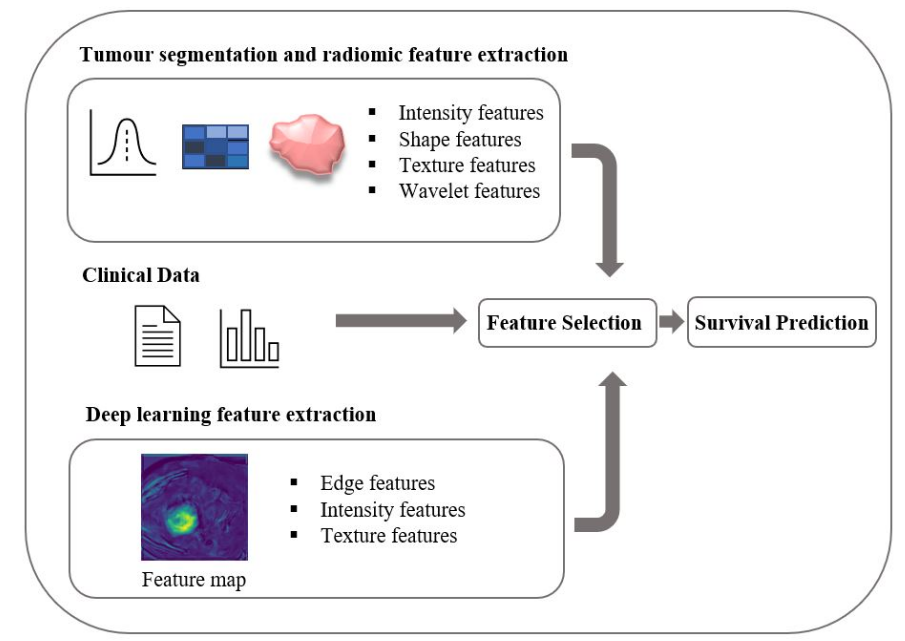
\includegraphics[scale=0.49]{annot6_features.jpg} \\
    \caption{\scriptsize{Пайплайн для задачи предсказания выживаемости. Состоит из трех шагов:
    сбор клинических данных, изображений и препроцессинга. Затем, выбираются извлеченные признаки и производится 
    предсказание выживаемости.}}
\end{center}
\end{minipage}


\subsubsection*{Модель для сегментации}
Архитектура предложенной сети NormResSE-UNet3+: 
\begin{itemize}
    \item На вход подается тензор, размерности 2x144x144x144, состоящий из конкатенации
    ПЭТ и КТ изображений.
    \item Энкодер состоит из residual squeeze-and-excitation блоков, первый блок из которых 
    содержит 24 фильтра. Размерность выхода энкодера - 384x3x3x3
    \item Путь декодирования состоит из полномасштабных соединений и модуля, содержащего 
    правильную разметку изорбражений (ground truth).
    \item У декодера одноканальный выход размерности 1х144х144х144
\end{itemize}



    \begin{minipage}{1.0\linewidth}
        \begin{center} 
        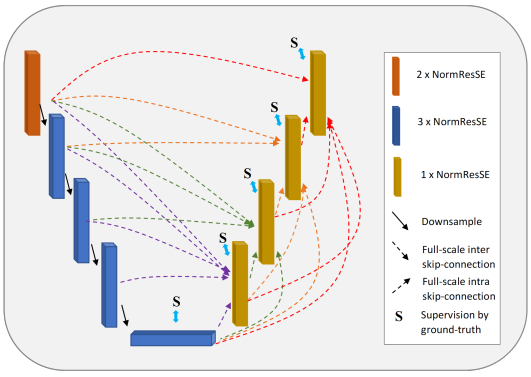
\includegraphics[scale=0.5]{ann6_arch.png}\\
        \caption{\scriptsize{Архитектура NormResSE-UNet3+}}
        
     \end{center}

    \end{minipage}

\subsection*{Данные}
Данные были предоставленны организаторами соревнования HECTOR - MICCAI. Всего 
тренировочных примеров - 224 из 5 центров: CHGJ, CHMR, CHUS,CHUP,CHUM.

\subsection*{Результаты}
Было обучено несколько моделей нейронных сетей для задачи сегментации опухолей головы и шеи. 
Результаты сведены в единую таблицу.
\begin{minipage}{1.0\linewidth}
    \begin{center}
        
    
    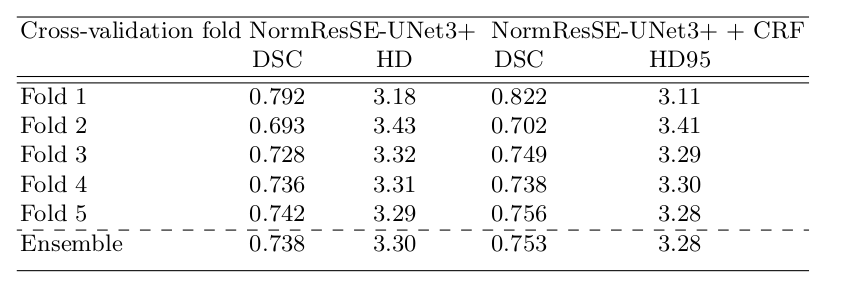
\includegraphics[scale=0.5]{ann6_res.png}\\
    \caption{\scriptsize{Количественные результаты сегментации}}
\end{center}
\end{minipage}
\\

Результаты предсказания выживаемости. Предложенная регрессионная модель CoxPH показала 
лучший результат: \\
\\
\begin{minipage}{1.0\linewidth}
    \begin{center}
        
   
    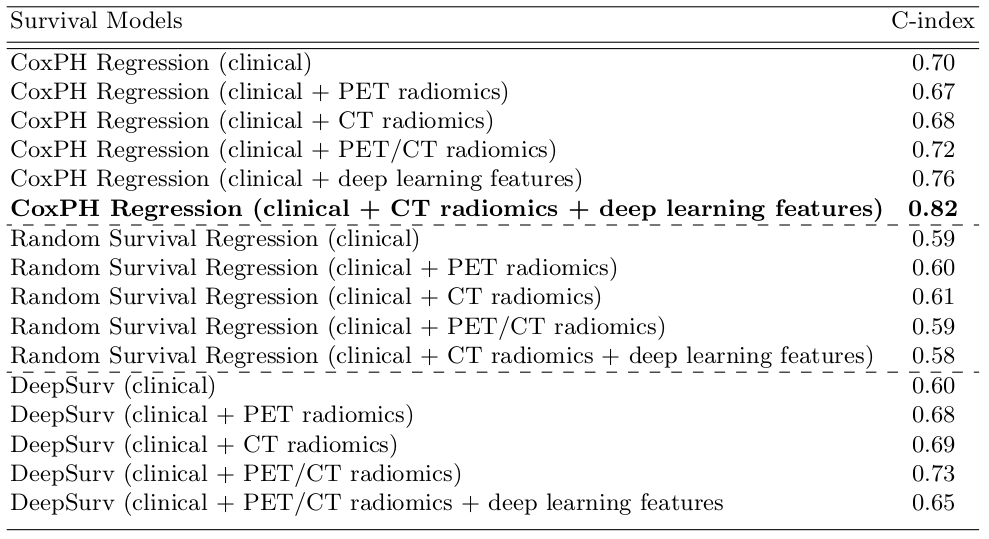
\includegraphics[scale=0.5]{ann6_reg_res.png}\\
    \caption{\scriptsize{Количественные результаты предсказания выживаемости.}}
\end{center}
\end{minipage}


\subsection*{Заключение}
Авторы предложили модель NormResSE-UNet3+ для сегментации опухолей головы и шеи по мультимодальным 
ПЭТ/КТ изображениям, в основе которой лежит архитектура UNet3+ с комбинированными слоями 
сжатия (squeeze-and-excitation), чтобы использовать возможности модели непрерывно фокусироваться 
на релевантных областях интереса, что помогло улучшить точность сегментации.

    \subsection*{Glioma Segmentation with Cascaded Unet}

% \subsection*{Ссылка} \url{https://arxiv.org/abs/1810.04008}
\subsubsection*{Введение}
Точная сегментация и реконструкция медицинских 3D изображений способны дать 
больше необходимой информации о прогрессировании заболевания и позволяют терапевту 
спланировать успешный курс лечения для больного. В данной работе \cite{Cascaded} авторы представляют
каскадный вариант популярной сети UNet \cite{Unet}, который итеративно улучшает результаты сегментации, 
полученные на предыдущих шагах. \par
\subsubsection*{Основная идея}
Предложенный метод может быть представлен как цепь классификаторов 
\(C_i\), одинаковой топологии F, у каждого из которых свой собственный 
набор параметров \(W_i\) для оптимизации в течение обучения.
Результат вычисления \(i\)-го шага представляется следующим образом: 
\(Y_i=F(X_i,Y_{i-1}, Y_{i-2}, W_i)\). Каждый из базовых блоков \(C_i\) - это
сеть архитектуры UNet, измененная для задачи сегментации глиом. В сравнении 
со стандартной архитектурой UNet, в предложенной модели используется несколько 
энкодеров, которые раздельно обрабатывают входные данные. Также, предложен метод объединения 
их выхода: в UNet \(i\)-й выход декодера зависит от выхода соответствующего 
энкодера и выхода предыдущего декодера - \(d_i^{t}=f(e_i^{t}, d^{t}_{i-1})\). 
Раскрывая первую свертку \(f\), получаем - \(d_i^{t}=g(W_{i,e}^{t}e_i^{t}+W_{i},d^{t}d^{t}_{i-1})\).
Далее предлагается объединить контекст, полученный на более низких слоях, 
добавляя соответствующий выход \(y^t\), поэтому \(d_i^{t}=g(W_{i,e}^{t}e_i^{t}+W_{i,d}^{t}d^{t}_{i-1}+W_{i,y}^{t}y^{t-i})\).
\\
\begin{minipage}{1.0\linewidth}
    \begin{center}
        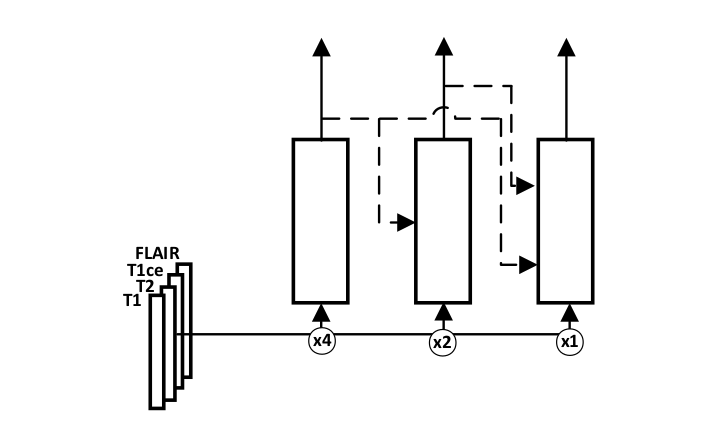
\includegraphics[scale=0.6]{ann7_arch.png} \\
        \captionof{figure}{\scriptsize{Схематическое представление метода, описанного в статье.
        T1, T2, T1ce, FLAIR - входные модальности МРТ-изображения, x4,x2 - понижающий
        фактор входа сети. Пунткирные линии - соединения между блоками \(C_i\).}}
    \end{center}
\end{minipage}

\subsubsection*{Результаты}

Результат сегментации  оценивался по метрике Dice, отдельно вычисленной
для следующих частей опухоли: WT (whole tumor) -  вся опухоль, ET (enchancing tumor) - 
усиливающаяся часть опухоли и TC (tumor core) - ядро опухоли. \\
 
\begin{center}
    \captionof{table}{Результаты без аугментации выходов}
\begin{tabular}{|c|c|c|c|}
    \hline
    Method & WT & ET & TC\\
    \hline
    UNet & 0.901 & 0.779 & 0.837 \\
    ME UNet & 0.907 & 0.784 & 0.827\\
    C ME UNet & 0.908 & 0.784 & 0.844\\
    \hline
\end{tabular}

\end{center}



\begin{center}
    

\captionof{table}{Результаты с аугментацией выходов}
\begin{tabular}{|c|c|c|c|}
\hline
Method & WT & ET & TC\\
\hline
UNet & 0.901 & 0.779 & 0.837 \\
ME UNet & 0.907 & 0.784 & 0.827\\
C ME UNet & 0.908 & 0.784 & 0.844\\
\hline
\end{tabular}

\end{center}


\subsubsection*{Заключение}

В данной работе был предложен алгоритм автоматической сегментации 
опухолей головного мозга по МРТ-зображениям, который решает также проблему
мультимодального входа и показывает хорошие резльтаты по сравнению с моделью UNet.



    
\section{CaraNet: Context Axial Reverse Attention Network for Segmentation of Small Medical Objects}

\subsection*{Ссылка} \url{https://arxiv.org/abs/2108.07368}
\subsection*{Введение}
 На данный момент разработано достаточное количество архитектур 
 сверточных сетей для решения задачи сегментации медицинских, которые 
 показывают хорошие результаты. Однако, только малая часть 
 исследований учитывает размер интересующих объектов на изображении
 и поэтому многие модели показывают плохой результат при сегментации
 объектов малого размера, что сильно влияет при диагностике заболевания.
 В данной работе предлагается нейросетевая модель Context Axial
 Reserve Attention Network (CaraNet), которая способна улучшить 
 результаты сегментации малых объектов по сравнению с уже существующими
 моделями.
\subsection*{Основная идея}
В архитектуре CaraNet используется параллельный частичный декодер 
(parallel partial decoder) для генерации высокоуровневой семантической
карты и набор операций (Context and Axial Reverse Attention) для 
идентификации глобальных и локальных признаков. 
\\Модули CaraNet:
\begin{itemize}
    \item \textit{Parallel partial decoder.} Эксперименты показали,
    что низкоуровненвые признаки вычислительно более сложны и вносят 
    меньший вклад в улучшение результатов сегментации. Поэтому, авторы 
    используют параллельный частичный декодер \(p_d(\cdot)\) для извлечения 
    высокоуровневых признаков \(PD=p_d(f_3,f_4,f_5)\) и получения глобальной карты 
    \(S_g\) из частичного декодера.
    \item \textit{Context module.} Чтобы получить контекстную информацию из высокоуровневых
    признаков, применяется модуль CFP (Channel-wise Feature Pyramid) cо степенью растяжения 
    (dilation rate) \(d=8\). После контекстного модуля можно получить многомасштабные 
    высокоуровневые признаки \(\{f_{3}^{'}, f_{4}^{'}, f_{5}^{'}\}\).
    \item \textit{Axial reverse attention.} Данный модуль состоит из двух частей:
    маршрут по оси (axial attention route) и обратный маршрут (reverse attention route). Глобальная 
    карта \(S_g\) может поймать только приблизительное расположение тканей без структурных деталей, 
    поэтому структурированный регион тканей постепенно добывается стиранием переднего плана 
    объекта с помощью операции reverse attention: \(R_{i}=1-Sigmoid(S_{i})\). По другому 
    маршруту применяется axial attention. Здесь сеть может извлечь глобальные зависимости и 
    локальное представление совершая вычисления по горизонтальной и вертикальной оси. 
\end{itemize}
\begin{minipage}{1.0\linewidth}
    \begin{center}
        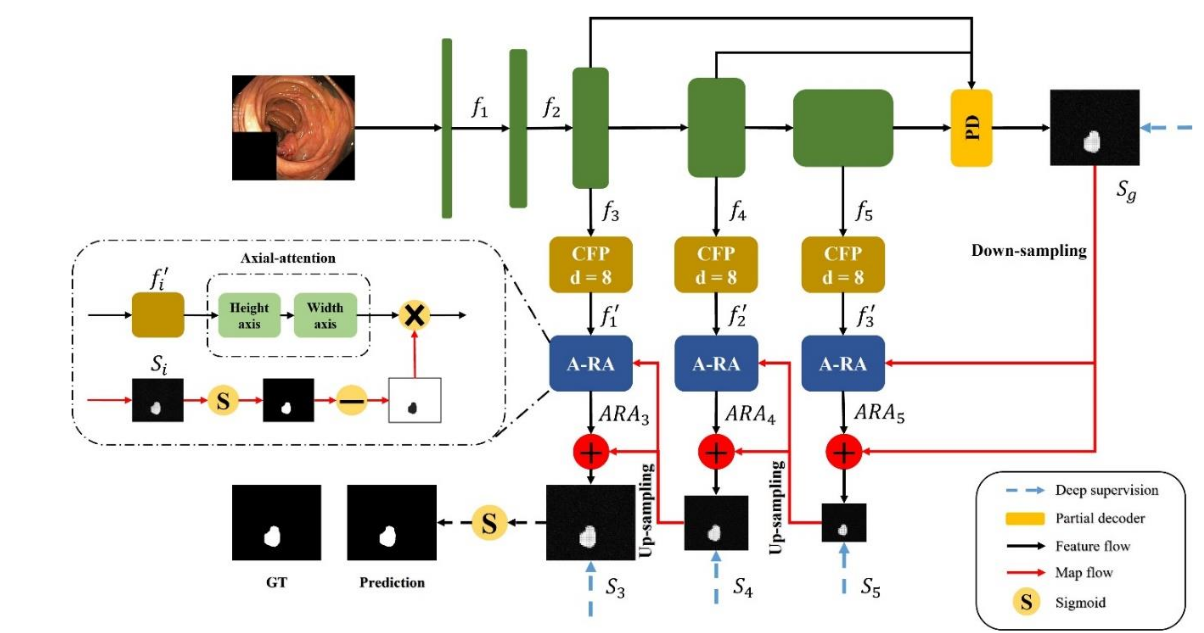
\includegraphics[scale=0.35]{ann8_arch.png} \\
        \caption{\scriptsize{Архитектура CaraNet, состоящая из трех контекстных модулей (CFP) и 
        модулей axial reverse attention (A-RA). 'S' - сигмоида.}}
    \end{center}
    
\end{minipage}
\subsection*{Данные}
\begin{itemize}
    \item BraTS 2018 - опухоли ГМ
    \item Kvasir-SEG, CVC-ColonDB, CVC-ClinicDB, CVC-
    300 and ETIS-LaribPolypDB - полипы
\end{itemize}
 
\subsection*{Результаты}
По сегментации полипов на основе пяти датасетов, предложенная модель CaraNet не только 
превосходит сравниваемые модели по общей производительности, но и на примерах с полипами 
малых размеров. \\
\\
\begin{minipage}{1.0\linewidth}
    \begin{center}
        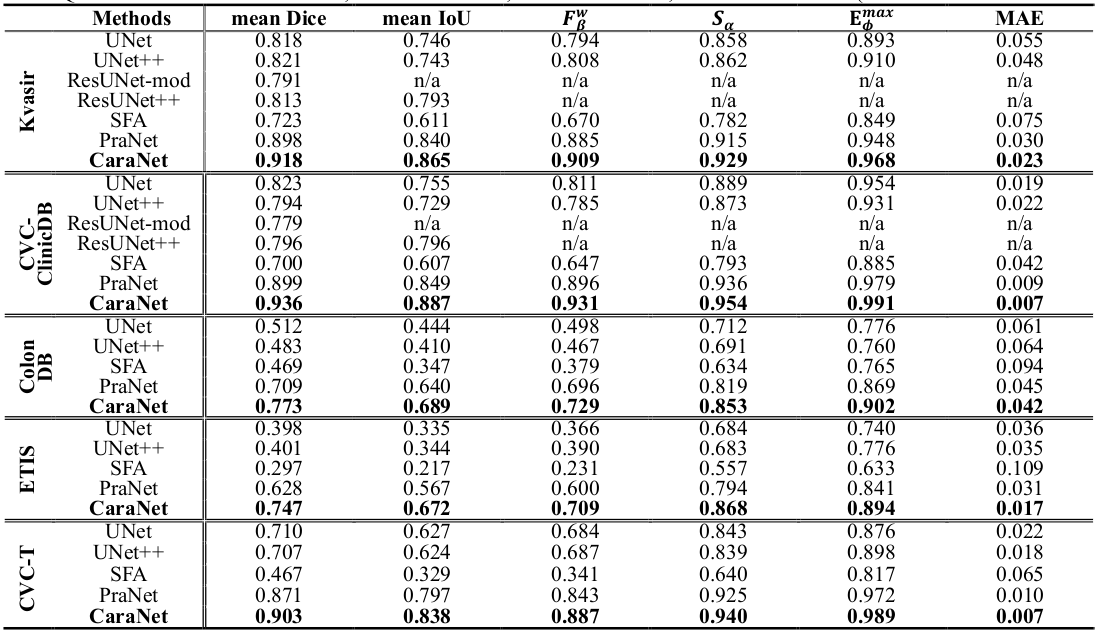
\includegraphics[scale=0.4]{ann8_res1.png}
        \caption{\scriptsize{Количественные результаты на Kvasir, CVC-ClinicDB, CVC-ColonDB, ETIS и CVC-T}}
    \end{center}
\end{minipage}

Для дальнейшей оценки эффективности сегментации малых объектов с помощью CaraNet был 
проведен еще один эксперимент, уже с участием опухолей ГМ из датасета BraTS 2018. CaraNet 
была сравнена с PraNet и показала лучший результат особенно в случаях с очень малыми объектами. \\
\\
\begin{minipage}{1.0\linewidth}
    \begin{center}
        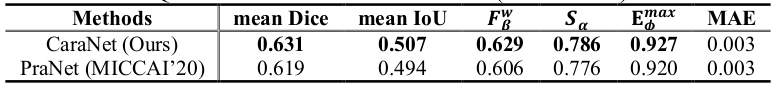
\includegraphics[scale=0.5]{ann8_res2.png} \\
        \caption{\scriptsize{Количественные результаты на датасете BraTS 2018}}
    \end{center}
    
\end{minipage}



\subsection*{Заключение}
Была предложена новая нейросетевая модель CaraNet, состоящая из комбинации моделей 
Axial Reverse Attention и Channel-wise Feature Pyramid, которая показала 
лучшие результаты сегментации малых объектов на медицинских изображениях по сравнению с уже существующими моделями 
UNet, UNet++, ResUNet-mod, ResUNet++, SFA, PraNet, что может внести большой вклад 
при постановке диагноза и выборе дальнейшей тактики лечения.
    \subsection*{Direct PET Image Reconstruction Incorporating Deep Image Prior and a Forward Projection Model}
% \subsection*{Ссылка} \url{https://arxiv.org/abs/2109.00768}
\subsubsection*{Введение}
Для того, чтобы снизить уроень радиации, поглощаемый пациентом при обследовании, 
проводят ПЭТ-визуализацию с низкими дозами облучения, что в свою очередь негативно влияет на 
зашумленность изображения. Существуют различные методы по постобработке ПЭТ-изображений,
такие как шумоподавление и восстановление для улучшения качества снимков при распознавании 
малых образований и количественном анализе. В данной работе \cite{ann9} предлагается метод
прямого восстановление ПЭТ-изображения, включающий в себя DIP фреймворк.
Алгоритм включает в себя модель прямой проеккции в функции потерь, чтобы достичь 
прямой реконструкции ПЭТ-изображения из синограм без учителя. 
\subsubsection*{Основная идея}
Модель прямой проекции ПЭТ может быть выражена так, что проектируемые данные \(y\in\mathbb{R}^{Mx1}\) связаны 
с пространственным распределением радиоактивного индикатора \(x\in\mathbb{R}^{Nx1}\) посредством афинного 
преобразования \(y=Px\), где \(P\in\mathbb{R}^{MxN}\) - матрица проекции, которая 
отражает вклад каждого вокселя в каждую линию ответа (line of response, LOR).
Реконструируемое изображение \(x\) вычисляется с помощью DIP фреймворка
следующим образом: \(x=f(\Theta|z)\), где \(f\)- это CNN, \(\Theta\) - веса CNN, а 
\(z\) - предыдущий входной вектор CNN. В данной работе для вычисления реконструированного 
изображения напрямую предлагается модель прямой проекции \(P\), втсроенная в функцию потерь. Была 
использована модель, основанная на 3D UNet и адаптированная под текущую задачую

\begin{minipage}{1.0\linewidth}
    \begin{center}
        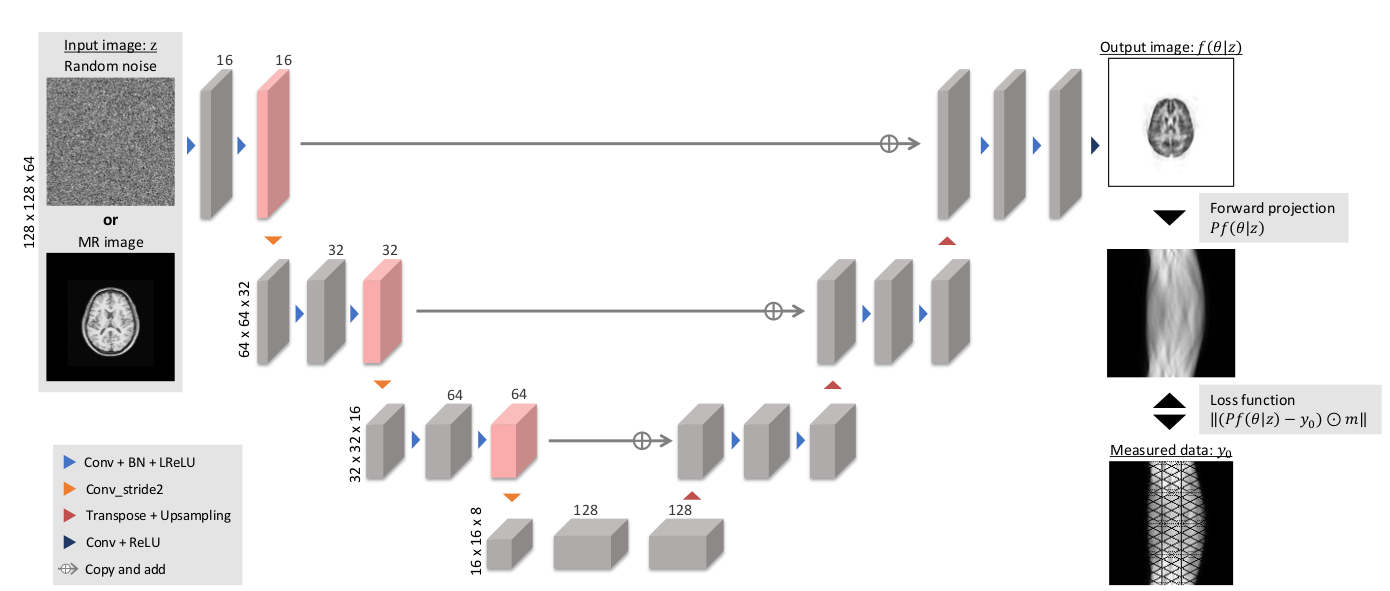
\includegraphics[scale=0.3]{ann9_arch.png} \\
        \captionof{figure}{\scriptsize{Общий вид предложенной модели прямой реконструкции ПЭТ.}}
    \end{center}
    
\end{minipage}

\subsubsection*{Данные} BrainWeb и созданные данные по методу Монте-Карло.
\subsubsection*{Результаты}
Был проведен сравнительный анализ предложенного метода
с методом filtered back projection (FBP) с использованием фильтра 
Ханна и Гаусса, а также с методом ML-EM. Показано, что описанный в статье метод
используя случайный шум и МРТ-изображение точно реконструирует ПЭТ-изображение 
без сокрытия или потерь информации в сравнении с методами FBP и ML-EM.
Основное ограничение данного исследования состоит в том, что оценивался 
только датасет ПЭТ изображений, полученных с радиоактивной меткой ФДГ.

\begin{minipage}{1.0\linewidth}
    \begin{center}
        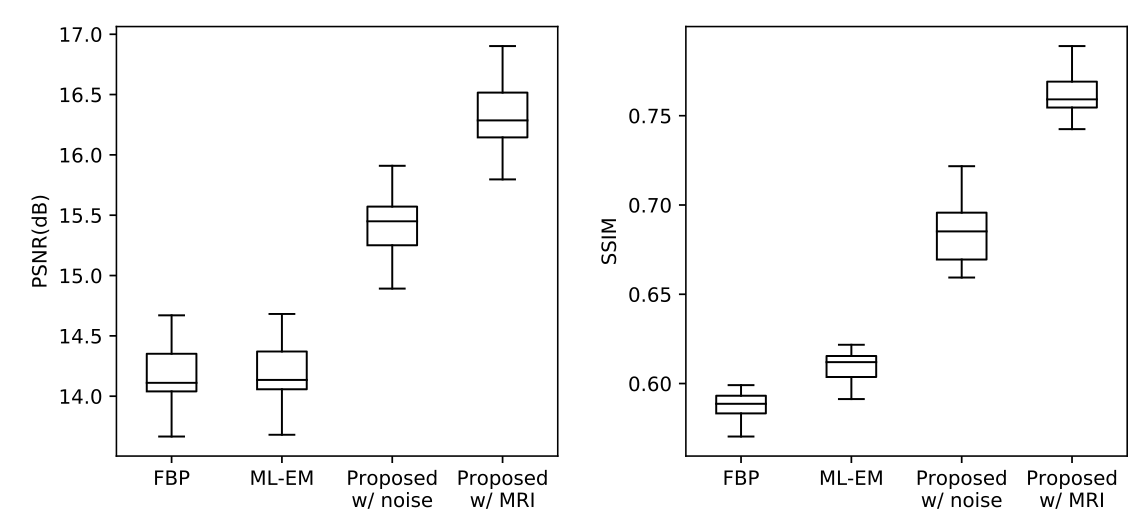
\includegraphics[scale=0.3]{ann9_res.png} \\
        \captionof{figure}{\scriptsize{Количественные результаты реконструированных
        изображений по метрике PSNR(слева) и SSIM(справа) относительно различных алгоритмов.
        Линия внутри прямоугольника представляет медиану, верхние и нижние линии прямоугольника - 
        75-й и 25-й перцентили соответственно. Верхние и нижние \glqq антенны\grqq представляют максимум и минимум соответственно.
        }}
    \end{center}
    
\end{minipage}
\subsubsection*{Заключение}
В сравнении с традиционными алгоритмами FBP и ML-EM, предложенный
метод показал лучший результат по метрикам PSNR и SSIM на данных, смоделированных с
использованием ФДГ.
    \subsection*{Virtual PET Images from CT Data Using Deep
Convolutional Networks: Initial Results}

% \subsection*{Ссылка}\url{https://arxiv.org/abs/1707.09585}
\subsubsection*{Введение}
Несмотря на то, что ПЭТ-исследования имеет большое количество положительных 
сторон, у него так же есть и недостатки - радиоактивный компонент опасен 
для беременных и кормящих женщин. Также, ПЭТ - сравнительно новый метод, который все 
еще является дорогостоящим для среднестатистического человека, также возможность получить 
ПЭТ обследование есть не во всех медицинских центрах. Сложность получения ПЭТ-изображений для 
поcледующего лечения послужила возникновению идеи поиска альтернативы - менее дорогостоящего, быстрого 
и легко в применении ПЭТ-подобного изображения. В данной работе \cite{ann10} исследуется 
модуль для создания виртуальных ПЭТ-изображений на основе информации из КТ-изображений.
\subsubsection*{Основная идея}
Фреймворк включает в себя три модуля:
\begin{itemize}
    \item Тренировочный модуль, который также включает в себя предобработку данных;
    \item Тестовый модуль, на вход которому подается КТ-изображение для предсказания 
    ПЭТ-подобного изображения на выходе;
    \item Модуль смешения (blending module), который соединяет выходы FCN и GAN.
\end{itemize}
FCN и GAN участвуют как в тренировке, так и в тестировании.

\begin{minipage}{1.0\linewidth}
    \begin{center}
        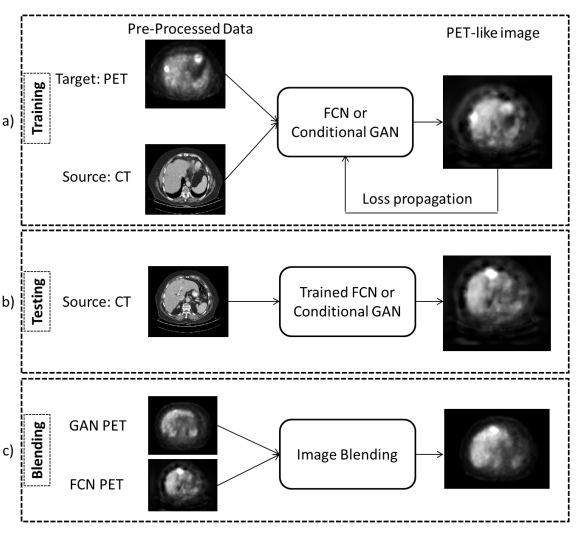
\includegraphics[scale=0.7]{ann10_sys.png} \\
        % \caption{\scriptsize{Предложенная система по созданию виртуальных ПЭТ-изображений.}}
    \end{center}
    
\end{minipage}
\\
\\
\\
Так как GAN обучается созданию реалистичных ПЭТ-изображений, результат его 
работы был намного ближе к реальным ПЭТ-изображениям, чем у FCN, который воспроизвел 
размытые изображения. Однако, FCN показал лучший результат на злокачественных
образованиях, чем GAN. Авторы использовали достоинства каждого метода, чтобы создать 
смешанное изображение, которое соединяет в себе реалистичность от GAN и более точный ответ 
о злокачественности от FCN. Сперва создается маска из выходного изображения FCN, которое 
содержит регионы с повышенным SUV (>2.5). По этой маске берется часть изображения из FCN, а 
остальная достраивается из изображения от GAN.

\subsubsection*{Данные}
Датасет включает в себя ПЭТ изображения печени (с опухолями и без) и соответствующие им
КТ изображения из Медицинского центр имени Хаима Шибы  (Израиль).
\subsubsection*{Результаты}
Сгенерированные ПЭТ-изображения были визуаьлно оценены радиологом и сравнены с реальными ПЭТ-изображениями
для распознавания опухолей печени. Распознанный регион считается опухолью, если он имеет 
значени \(SUV_{max}>2.5\).  Для оценки были вычислены значения TPR и FPR.
Система успешно распознала 24 из 26 опухолей (TPR 92.3\%), c только 
двумя ложноположительными ответами среди всех 8 сканов (FPR 0.25).
\\
\\
\\
\begin{minipage}{1.0\linewidth}
    \begin{center}
        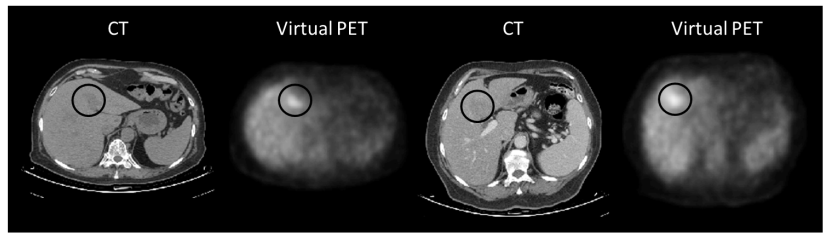
\includegraphics[scale=0.5]{ann10_res2.png} \\
        % \caption{\scriptsize{Ложноположительные результаты выделены черным кругом.}}
    \end{center}
    
\end{minipage}
\subsubsection*{Заключение}
Была разработана система создания виртуальных ПЭТ-изображений 
по КТ изображениям с использованием FCN и GAN, которая показала 
сравнительно хорошие результаты. Работа интересная, однако, сложно представить 
ее использование в реальной жизни и степень востребованности и доверия к методу.
}


% Информация о годе выполнения работы
\def\Year{%
    % 2006%
    \the\year%     % Текущий год
}

% Укажите тип работы
% Например:
%     Выпускная квалификационная работа,
%     Магистерская диссертация,
%     Курсовая работа, реферат и т.п.
\def\WorkType{%
    % Выпускная квалификационная работа%
    % Магистерская диссертация%
    % Курсовая работа%
    % Реферат%
    %Дипломная работа%
    Аннотации статей
}

% Название работы
%%%%%%%%%%% ВНИМАНИЕ! %%%%%%%%%%%%%%%%
% В МГУ ОНО ДОЛЖНО В ТОЧНОСТИ
% СООТВЕТСТВОВАТЬ ВЫПИСКЕ ИЗ ПРИКАЗА
% УТОЧНИТЕ НАЗВАНИЕ В УЧЕБНОЙ ЧАСТИ
\def\Title{%
    Разработка методов искусственного интеллекта для дифференциальной диагностик
    глиальных опухолей по данным динамических позитронно-эмиссионных исследований.%
}


% Имя автора работы
\def\Author{%
    Айрапетьянц Каринэ Арсеновна%
}


% Информация о научном руководителе
%% Фамилия Имя Отчество%
\def\SciAdvisor{%
    Малоян Нарек Гагикович%
}
%% В формате: И.~О.~Фамилия%
\def\SciAdvisorShort{%
    Н. ~Г. ~Малоян%
}
%% должность научного руководителя
\def\Position{%
    % профессор%
    %доцент%
    % старший преподаватель%
    % преподаватель%
    % ассистент%
    % ведущий научный сотрудник%
    % старший научный сотрудник%
    % научный сотрудник%
    % младший научный сотрудник%
}
%% учёная степень научного руководителя
\def\AcademicDegree{%
    % д.ф.-м.н.%
    % д.т.н.%
   %к.ф.-м.н.%
    % к.т.н.%
    %без степени%
}

% Информация об организации, в которой выполнена работа
%% Город
\def\Place{%
    Москва%
}
%% Университет
\def\Univer{%
    Московский государственный университет имени М.~В.~Ломоносова%
}
%% Факультет
\def\Faculty{%
    Факультет вычислительной математики и кибернетики%
}
%% Кафедра    
\def\Department{%
    Кафедра информационной безопасности%
}     

%%%% Переключите статус документа для отладки
%%%% В режиме draft документ собирается очень быстро
%%%% и выводится полезная информация о том
%%%% какие строки вылезают за границы документа, что удобно для борьбы с ними
\def\Status{%
    % draft%
    final%
}

%%%% Включает и выключает подпись <<С текстом работы ознакомлен>>
\def\EnableSign{%
    % true%
}
